\section{Background}
\subsection{Importance of accessibility studies}
\justify

% Potentiaalisesti hyödyllisiä linkkejä Helsingin autoilusta
%https://www.hel.fi/hel2/Helsinginseutu/HS_tunnusluvut/liikennemaara_ja_autonomistus.pdf
%https://www.hsl.fi/sites/default/files/19_2016_auton_omistus_helsingin_seudulla.pdf
%https://www.hsl.fi/tutkimukset/muut-selvitykset
%https://www.hel.fi/helsinki/fi/kartat-ja-liikenne/kadut-ja-liikennesuunnittelu/tutkimus-ja-tilastot/moottoriajoneuvoliikenteen-maarat/
%https://www.hel.fi/helsinki/fi/kartat-ja-liikenne/kadut-ja-liikennesuunnittelu/tutkimus-ja-tilastot/liikenteen-sujuvuus/
%http://pxnet2.stat.fi/PXWeb/pxweb/fi/StatFin/StatFin__lii__mkan/
%https://julkaisut.vayla.fi/pdf8/lti_2018-01_henkiloliikennetutkimus_2016_web.pdf
%--liikkumistottumukset
%https://www.hsl.fi/sites/default/files/hsl_julkaisu_9_2019_netti.pdf 
%-- autojen määrä viime vuosikymmeninä suomessa
%https://www.stat.fi/til/mkan/2019/mkan_2019_2020-02-28_tie_001_fi.html

\begin{itemize}
    \item Donald Shoup searching for parking
    \item city congestion
    \item private car mobility
    \item amount of cars in urban settings
    \item the space parked cars take
\end{itemize}

The Helsinki Capital Region faces increasing pressure to manage its traffic because (\textcolor{red}{LÄHDE}).

%tsek helsingin raportit ja HLT, sitten päätä mitä päätä mitä kirjoitat
A high-performance public transport system operates in the Helsinki Capital Region and is comprised of buses, train, subway, and tram. In 2017, the subway expanded from Helsinki to Espoo, triggering a new phase of quickly evolving cityscape in the surroundings of the new stations. A host of large scale additions to the system are being planned, with some, like Jokeri Light Rail, already in construction. Despite the extensive service level of Helsinki Capital Region public transport, households especially in Espoo, Vantaa, and Kauniainen remain dependent on personal vehicles (\textcolor{red}{cite}).

\begin{hyphenrules}{nohyphenation}
    \begin{table}[H]
        \centering
        \def\arraystretch{1.2}
        \setlength\tabcolsep{1.2ex}
        \caption[Amount of cars registered in Helsinki Capital Region and in Finland total]{The number of private cars registered in the Helsinki Capital Region municipalities, in KUUMA municipalities, and in Finland total (\cite{StatisticsFinland2020b}). Private cars decommissioned from traffic are not included in this table.} 
        \label{tab:registered_cars}
        \begin{tabular}{ llll @{} >{\raggedleft\arraybackslash}p{2cm} @{} }
            \toprule
                                            & 2011      & 2015      & 2019      & Growth 2011--2019 \\
            \midrule
            Helsinki                        & 207 639   & 206 229   & 214 583   & 3.2 \% \\
            Espoo                           & 107 833   & 115 446   & 122 185   & 11.7 \% \\
            Vantaa                          & 91 844    & 98 963    & 109 068   & 15.8 \% \\
            Kauniainen                      & 3 815     & 4 105     & 4 324     & 11.8 \% \\
            \greyrule
            KUUMA municipalities*           & 149 930   & 157 984   & 169 760   & 11,7 \% \\
            \greyrule
            Finland                         & 2 978 729 & 3 257 581 & 3 574 570 & 16.7 \% \\
            \bottomrule
            \multicolumn{5}{ p{12cm} }{\textsuperscript{*}\footnotesize{KUUMA municipalities are the Greater Helsinki municipalities without the Helsinki Capital Region: Hyvinkää, Järvenpää, Kirkkonummi, Kerava, Mäntsälä, Nurmijärvi, Pornainen, Sipoo, Tuusula, and Vihti (\cite{KUUMA-seutuliikelaitos2020}).}}
        \end{tabular}
    \end{table}
\end{hyphenrules}

% tarkempaa aineistoa autotiheydestä:
%https://www.hel.fi/hel2/helsinginseutu/hs_tunnusluvut/liikennemaara_ja_autonomistus.pdf
\begin{hyphenrules}{nohyphenation}
    \begin{table}[H]
        \centering
        \def\arraystretch{1.2}
        \setlength\tabcolsep{1.2ex}
        \caption[Density of private cars in Helsinki Capital Region in 2019]{Density of private cars in Helsinki Capital Region municipalities, in KUUMA municipalities, and in the entire Finland in 2019 (\cite{StatisticsFinland2020}, \citeyear{StatisticsFinland2020b}). Private cars decommissioned from traffic are not included in this table.} 
        \label{tab:car_density}
        \begin{tabular}{ l @{} >{\raggedleft\arraybackslash}p{2cm} >{\raggedleft\arraybackslash}p{2cm} >{\raggedleft\arraybackslash}p{3.5cm} @{} }
            \toprule
                                            & Population 2019   & Private cars 2019 & Private car density (cars/1000 inhabitants) \\
            \midrule
            Helsinki                        & 656 970           & 214 583           & 326 \\
            Espoo                           & 291 490           & 122 185           & 419 \\
            Vantaa                          & 236 434           & 109 068           & 462 \\
            Kauniainen                      & 9 990             & 4 324             & 432 \\
            \greyrule
            KUUMA municipalities*           & 326 211           & 169 760           & 520 \\
            \greyrule
            Finland                         & 5 532 333         & 2 745 074         & 496 \\
            \bottomrule
            \multicolumn{4}{ p{12cm} }{\textsuperscript{*}\footnotesize{KUUMA municipalities are the Greater Helsinki municipalities without the Helsinki Capital Region: Hyvinkää, Järvenpää, Kirkkonummi, Kerava, Mäntsälä, Nurmijärvi, Pornainen, Sipoo, Tuusula, and Vihti (\cite{KUUMA-seutuliikelaitos2020}).}}
        \end{tabular}
    \end{table}
\end{hyphenrules}

\newpage
\subsection{Accessibility studies in geography}
\justify

\begin{itemize}
  \item Benenson et al. research
\end{itemize}

\begin{figure}[H]%
    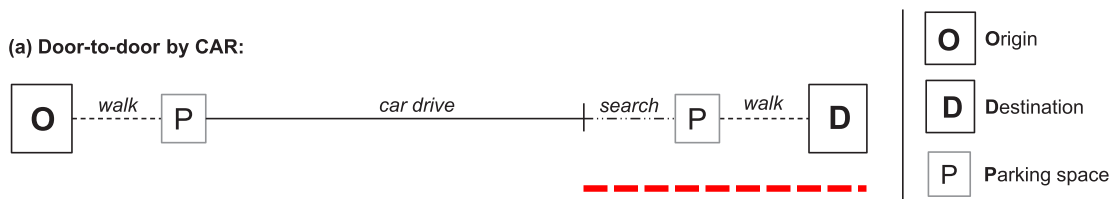
\includegraphics[width=\textwidth]{images/door2door.png}
    \caption[Door-to-door approach]{The entire travel chain of a private car using the door-to-door approach. The red dashed line represents the parking process segment of the travel chain. Figure adapted from Salonen and Toivonen (\citeyear{Salonen2013}).}%
    \label{fig:door-to-door}%
\end{figure}

\newpage
\subsection{Previous parking studies}
\justify

PARKFIT, an algorithm for estimating parking patterns (\cite{Levy2015}).

PARKAGENT, simulation that captures self-organising dynamics of "parking agents" (drivers) (\cite{Benenson2008}). Point out shortcomings in parking time estimations

Donald Shoup Cruising for Parking, High Cost of Free Parking

\newpage
\subsection{Parking time estimations}
\justify

\begin{itemize}
  \item Talk about Häyrynen \& Kalenoja's Tampere
  \item Broad estimations used in Helsinki Travel Time Matrix:
  \item 0.42 min searching for parking
  \item 2 min and 2.5 min walking in TTM18
  \item A word about donald shoup's findings
\end{itemize}

\newpage
\subsection{Research in parcipatory GIS and map surveys}
\justify

\begin{itemize}
  \item PPGIS bibliography and map survey options such as Survey123 and Maptionnaire
  \item Talk about own work on the map survey
  \item How did the map survey I created work for the purpose of collection user data
\end{itemize}